\section{Local Challenge: Passing Challenge}
\label{sec:PassingChallenge}

\subsection{Idea of the Challenge}
In recent year's teamwork has played an increasingly important role in the RoboCup SPL. A fundamental point in the development of this kind of strategy is the passing of the ball between teammates. The goal of this challenge is to push teams to develop an efficient system for the realization of an offensive strategy based on one or more passes between teammates. 

The setting of the challenge is so defined: there are two attackers robots, and two static obstacle robots as defenders (\cf Section \ref{sec:stationary_obstacle_robots}). The purpose of the attackers' robots is to execute the highest number of passes between them in a limited amount of time. The timeout is set to 5 minutes.
The referee will observe the challenge execution using video streaming, see \ref{sec:streaming_setup}.
Each team has three attempts on this challenge; the final score for every team is the one obtained in the best of the three attempts. Teams cannot change code between attempts.
\begin{figure}[ht]
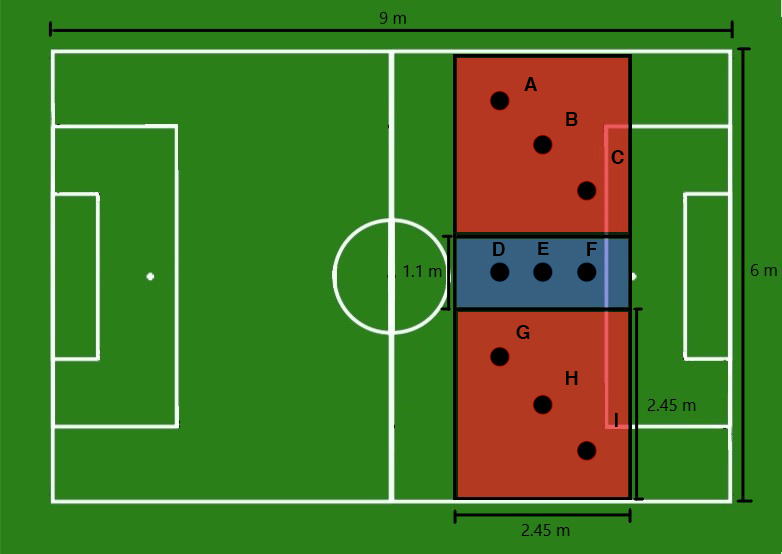
\includegraphics[width=0.95\linewidth]{figs/ch_2_full.jpg}
\caption{Full-size field setup. The red zone represents the movement areas of the attacking robots. The blue zone represents the defender's area. }
\label{ch2:zone96}
\centering
\end{figure}

\begin{figure}[ht]
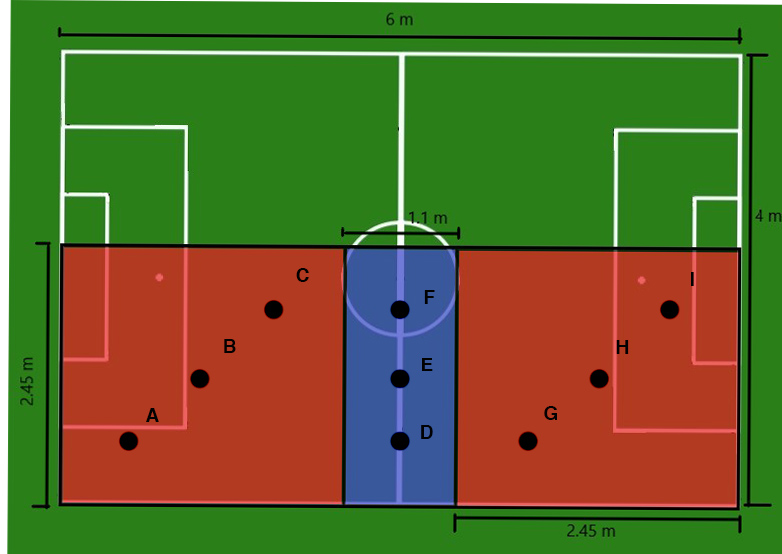
\includegraphics[width=0.95\linewidth]{figs/ch_2_reduced.jpg}
\caption{Reduced size field setup. This image shows the application of the challenge's zones on a 6m by 4m field. The red zone represents the movement areas of the attacking robots. The blue zone represents the defender's area.}
\label{ch2:zone64}
\centering
\end{figure}


\subsection{Field Setup}
This challenge is designed to be conducted independently within the individual labs of participating teams. The requirements are the presence of a half full-size field or any field capable of hosting the area required by the challenge, whose overall size is that of a rectangle measuring 6m by 2.45m.  
The divisions and dimensions of the zones of interest of the challenge for the full-size field is shown in Figure \ref{ch2:zone96}. In Figure \ref{ch2:zone64}, is instead shown the division of the zones on a 6m by 4m field.
The red zones represent the movement zones available to attacker robots. The blue zone represents the zone of placement of the defender robots.
Field areas should be made visible by demarcating them on the field through the use of tape of any color except white. Anyway, the lines must still be easily visible by the referee in streaming video.

\info[]{TODO: please consider specifying the tape color to be green and that no white lines should be broken by the green tape}

\info[]{TODO: please consider specifying how robots should know if they are inside the allwed/red area. Should they self-loclize using white field lines?}

\subsection{Robots positioning}
In order to participate each team has to provide four robots, two active ones and two inactive ones. The two active robots are the attacking robots. The defending robots act like static obstacle robots (\cf Section \ref{sec:stationary_obstacle_robots})
%TODO: Common Rules reference
Defenders must be turned off or otherwise placed out of the robots' communication network (for example, by setting them up as members of an opposing team).
The starting robot's positions are identified by the points ${A,B,C,D,E,F,G,H,I}$ in Figures \ref{ch2:zone96} and \ref{ch2:zone64}.

The robot's positions are:

\textbf{Full size field (Vertical setup) -} the reference frame of each point is put in the lower left corner of the corresponding area.
\\
$A = G = (0.6m, 1.8m)$
\\
$B = H = (1.2m, 1.2m)$
\\
$C = I = (1.8m, 0.6m)$
\\
$D = (0.6, 0.55m)$
\\
$E = (1.2m, 0.55m)$
\\
$F = (1.8m, 0.55m)$
\\
\\
\textbf{Reduced size field (Horizontal setup) -} the reference frame of each point is put in the lower left corner of the corresponding area.
\\
$A = G = (0.6m, 0.6m)$
\\
$B = H = (1.2m, 1.2m)$
\\
$C = I = (1.8m, 1.8m)$
\\
$D = (0.6, 0.55m)$
\\
$E = (1.2m, 0.55m)$
\\
$F = (1.8m, 0.55m)$
\\
\\
The attacking robots are placed in two random points between the positions A, B, C, for one robot and G, H, I, for the other one.  Randomly one of the two robots is selected as the initial bearer of the ball. The defenders are positioned randomly in two points selected between the D, E, F positions.
The points disposition is shown in Figure \ref{ch2:zone96} and Figure \ref{ch2:zone64}.
The Robots are directly put on the selected points while the GameController is in the state of "Initial". Then the GameController state will be put in "Ready" state and then in "Set". At this point the episode will start using the referee whistle and the GameController (as in the regular SPL games). 

\subsection{Passing definition}
For the correct evaluation of this challenge, it is essential to define the intended passing objectively. It is based on two fundamental requirements:
\begin{itemize}
    \item The ball has been touched by two robots of the same team,
    \item The ball moved more than one meter from its starting position.
    \item ToDo: A robot is not allowed to enter the blue area. (Otherwise it could dribble the ball into the other area. Ball is moved and in the end touched by another robot.)
\end{itemize}


\subsection{Episode definition}
Each episode starts with the referee's whistle. An episode can be concluded in four ways: 
\begin{itemize}
    \item[1] The timeout is reached,
    \item[2] The defenders touch the ball,
    \item[3] One attacker player stays out of its starting red area for more than 30 seconds.

\end{itemize}

\subsection{Points assignment and overall ranking}
The attacking team is awarded one point for each pass achieved (see rules above). If the ball ends out of the boundaries of the red area of the receiving robot after the pass no point is awarded. Each team will have three attempts on the challenge. Teams cannot do any modification to the code between the attempts. At the end of the three attempts the best score between them is selected as the team's score. The teams will be ranked by their score, from the highest to the lowest. 

\subsection{Additional Rules}
\begin{itemize}
    \item The attackers can leave the respective red rectangle zone for a maximum time of 30 seconds (in order to retrieve the ball and pass it back), then they have to come back inside the area.
    \item If during a pass the ball touches the defender, even if the ball doesn't stop, the challenge episode is however considered as finished
    \item If the ball ends out of the red areas, it is manually put back in a random point inside the closest red area by the referee.
    \item Points are counted by the referee
    
\end{itemize}
